\documentclass[12pt,twocolumn]{article}  % Change to report, book, etc. if needed

% Essential Packages
\usepackage[utf8]{inputenc}   % Handle UTF-8 encoding
\usepackage[T1]{fontenc}      % Proper font encoding
\usepackage{lmodern}          % Modern font
\usepackage{geometry}         % Page margins
\geometry{margin=1in}        % Set 1-inch margins

% Math and Symbols
\usepackage{amsmath, amssymb} % Math symbols and environments
\usepackage{physics}          % Common physics notation
\usepackage{siunitx}          % SI unit formatting

% Graphics and Figures
\usepackage{graphicx}         % Image inclusion
\usepackage[font=tiny]{caption, subcaption} % Better figure captions
\usepackage{float}            % Control float positioning
\usepackage{listings}
\usepackage{color}
\usepackage{tikz}
\usepackage{wasysym}
\usepackage{siunitx}
\usepackage{textcomp}
\usepackage{changepage}

\usepackage{minted}


\usetikzlibrary{positioning}
\usetikzlibrary{angles}
\usetikzlibrary{decorations.markings}

\lstset{language=Python}
\definecolor{dkgreen}{rgb}{0,0.6,0}
\definecolor{gray}{rgb}{0.5,0.5,0.5}
\definecolor{mauve}{rgb}{0.58,0,0.82}

\lstset{frame=top,
  language=Python,
  aboveskip=3mm,
  belowskip=3mm,
  showstringspaces=false,
  columns=flexible,
  basicstyle={\scriptsize\ttfamily},
  numbers=none,
  numberstyle=\tiny\color{gray},
  keywordstyle=\color{blue},
  commentstyle=\color{dkgreen},
  stringstyle=\color{mauve},
  breaklines=true,
  breakatwhitespace=true,
  tabsize=3
}


% Tables
\usepackage{booktabs}         % Better table formatting
\usepackage{array}            % Extended table options

% Title and Author
\title{Spacecraft Mission}
\author{Alex Freeman}
\date{\today}

\begin{document}

\maketitle


This report will cover all parts of assignment one in the Aerospace 720 course
\newline
\newline
In Two-body Orbital Dyanmics, Newton's Second Law of Motion applies. Equating forces
\begin{equation}
    \bar{F} = m\bar{a}
\end{equation}
\begin{equation}
    \bar{F} = \frac{Gmm}{r^2}\hat{r}
\end{equation}
Gives the equations of motion 
\begin{equation}
    \ddot{\bar{r}} = \frac{-\mu\cdot\bar{r}}{r^3}
\end{equation}

This can be represented by the simple diagram showing two bodies with different masses
where the arrows represent the position vectors involved.
\begin{center}
    

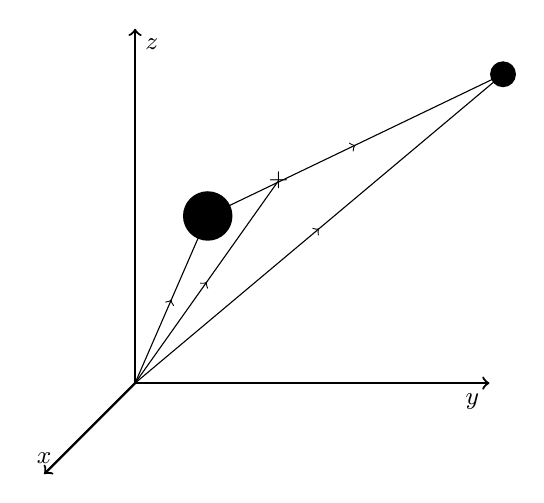
\begin{tikzpicture}
    [scale=1.5, every node/.style={font=\small}, 
    axis/.style={-, postaction={decorate},
    decoration={markings, mark=at position 0.5 with {\arrow{>}}}
    }]

    \def\x{1}
    \def\y{1.8}
    \def\z{1}


    % Draw the axes
    \draw[->, thick] (0,0,0) -- (3,0,0) node[anchor=north east]{$y$};
    \draw[->, thick] (0,0,0) -- (0,3,0) node[anchor=north west]{$z$};
    \draw[->, thick] (0,0,0) -- (0,0,2) node[anchor=south]{$x$};

    
    \draw[axis] (0,0,0) -- (\x,\y,\z);
    \draw[axis] (0,0,0) -- (3.5,3,1);
    \draw[axis] (\x,\y,\z) -- (3.5,3,1);
    \draw[axis] (0,0,0) -- (1.6,2.1,1);
    \node at (1.6,2.1,1) {$+$};

    \filldraw[fill=black, draw=black, thick] (\x,\y,\z) circle [radius=0.2];
    \filldraw[fill=black, draw=black, thick] (3.5,3,1) circle [radius=0.1];

  \end{tikzpicture}
\end{center}
\section{Orbital Propagation}
\subsection{Solving Kepler's Equation}

We need to solve Kepler's Equation using numerical methods. Using the Newton-Rasphon Method we can take the eccentricity and mean anamoly as 
inputs and numerically solve for the eccentric anamoly. 

\begin{lstlisting}
def Kepler(e, M, tol = 1e-12, max_i = 1000):
    E = M                               # Guess solution
    for i in range(max_i):
        f_E = E - e * np.sin(E) - M     # Define the function in terms of f(E) = 0
         f_prime = 1 - e * np.cos(E)    # Derive the function in terms of E
        del_E = f_E / f_prime           
        E_new = E - del_E               # Calculate the new eccentric anamoly
        if np.abs(del_E) < tol:         # If the value is within the set tolerance 
            theta = 2*np.arctan(np.tan(E_new/2) * ((1+e)/(1-e))**(0.5))
            return theta                # Return true anamoly
        E = E_new
\end{lstlisting}
\vspace{0.5cm}
If we set the tolerance to $1e-12$, we can compute the true anamoly of the asteroid 
at $t_0$ and $t_0 + 100$ days. A\_ae0 is the OBJ data of the asteroid, it is an array.
\begin{lstlisting}
trueAnamoly_asteroidt_0 = Kepler(A_ae0[2], A_ae0[6])  
meanAnamolyt_100 = get_mean_anamoly(100*(3600*24), A_ae0[6], A_ae0[1])
trueAnamoly_asteroidt_100 = Kepler(A_ae0[2], meanAnamolyt_100)
\end{lstlisting}
Printing these values gives that the true anamoly $\theta_{t_0} = 1.4246$ and $\theta_{t_0 + 100} = 2.1369$. 
Where these answers are in radians.

\vspace{0.5cm}
Now I have created a function that takes in a state of orbital elements and returns 
the position and velocity vectors at that point. It uses a rotation matrix to convert from 
the perifocal frame to the ECI frame. This is defined via $i, \omega$, and $\Omega$ terms and is 
calculated using the defind matricies in the appendix.
\begin{lstlisting}   
def COE2RV(arr, mu):
    a, e, i, Omega, omega, theta_var = arr[0:6]
    h = np.sqrt(mu * a * (1 - e**2))
    r = a*(1-(e**2))/(1 + e*np.cos(theta_var))

    arr_r = np.array([r*np.cos(theta_var), r*np.sin(theta_var), 0])
    arr_v = (mu/h)* np.array([-np.sin(theta_var), e + np.cos(theta_var), 0])

    # Rotate position and velocity from perifocal to inertial frame using the 
    # transfomration matrix
    R_matrix = rotation_matrix(i, Omega, omega)

    r_ijk = R_matrix @ arr_r
    v_ijk = R_matrix @ arr_v
    return r_ijk, v_ijk
\end{lstlisting}
\vspace{0.35cm}
Using this code we can output the state vector at some time $t$. The first three values 
are the $x,y,z$ positions in \textbf{km}. The last three are the velocity values in the $x,y,z$ direction 
in \textbf{km/s}.

\[
\begin{array}{c}
\textbf{At } t_0: \\
\mathbf{\bar{X}} =
\begin{bmatrix}
x = -1.1694365\mathrm{e}{+08} \\
y =  1.53462780\mathrm{e}{+08} \\
z = -6.7446087\mathrm{e}{+06} \\
v_x = -3.1710203\mathrm{e}{+01} \\
v_y = -3.6285380\mathrm{e}{+00} \\
v_z = -1.8931546\mathrm{e}{+00}
\end{bmatrix}
\\[7em] % small vertical space
\textbf{At } t_0 + 100: \\
\mathbf{\bar{X}} =
\begin{bmatrix}
x = -3.2057997\mathrm{e}{+08} \\
y =  6.72659396\mathrm{e}{+07} \\
z = -1.8991445\mathrm{e}{+07} \\
v_x = -1.6964807\mathrm{e}{+01} \\
v_y = -1.2943780\mathrm{e}{+01} \\
v_z = -1.0284663\mathrm{e}{+00}
\end{bmatrix}
\end{array}
\]


Next, I have written a function called "Ephemeris". It returns the position and velocity at some time t.
\begin{lstlisting}
def Ephemeris(t, OBJdata, mu):
    time, a, e, i, Omega, omega, mean_anamoly = OBJdata[0:7]
    nu_t = (mu / (a**3))**0.5
    t = t - t_0_days*days_convert
    mean_anamoly_t = mean_anamoly + nu_t * (t)

    h = np.sqrt(mu * a * (1 - e**2))
    theta_var = Kepler(e, mean_anamoly_t)
    r = a*(1-(e**2))/(1 + e*np.cos(theta_var))
    arr_r = np.array([r*np.cos(theta_var), r*np.sin(theta_var), 0])
    arr_v = (mu/h)* np.array([-np.sin(theta_var), e + np.cos(theta_var), 0])
    R_matrix = rotation_matrix(i, Omega, omega)
    r_ijk = R_matrix @ arr_r
    v_ijk = R_matrix @ arr_v
    
    return r_ijk, v_ijk
\end{lstlisting}

\noindent Using this code we can calculate the position and velocity vectors in the Sun's frame of reference. 


\begin{figure}[H]
    \centering
    \begin{minipage}{0.48\textwidth}
        \centering
        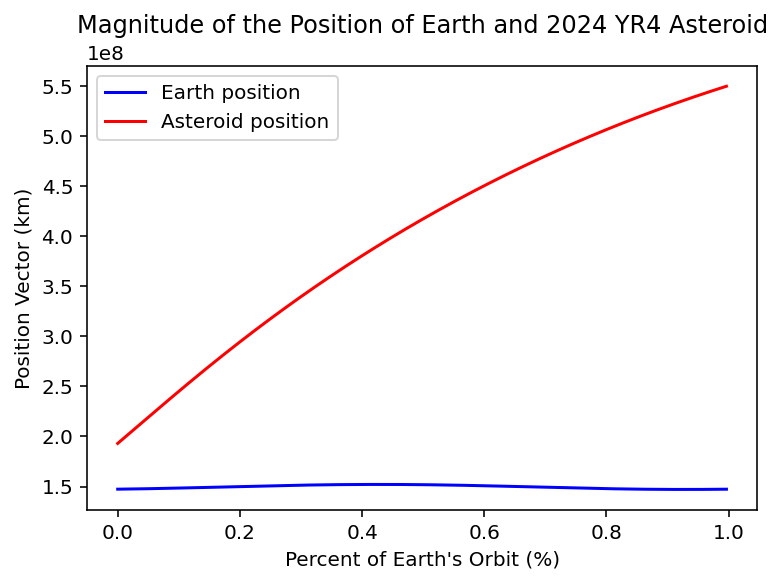
\includegraphics[width=\textwidth]{Images/114-pos.png}
        \caption{Position vectors of Earth and the Asteroid for a full Earth orbital period}
    \end{minipage}
    \hfill
    \begin{minipage}{0.48\textwidth}
        \centering
        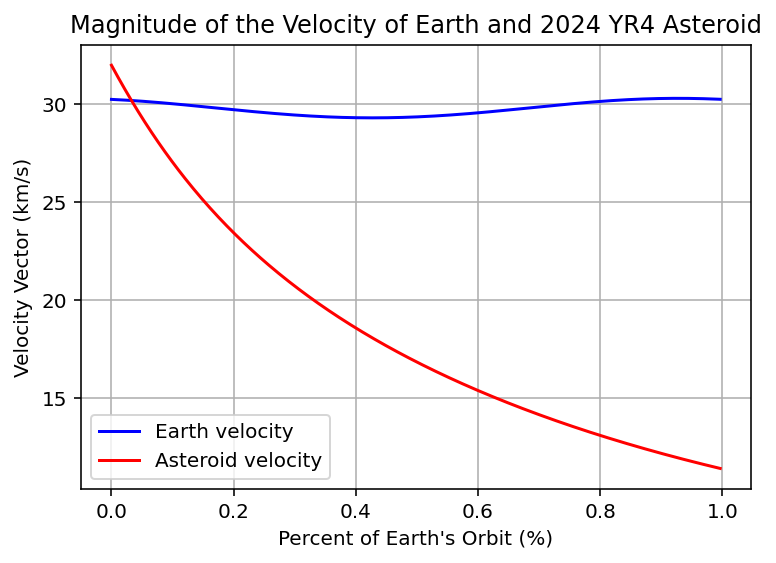
\includegraphics[width=\textwidth]{Images/114-vel.png}
        \caption{Velocity vectors of Earth and the Asteroid for a full Earth orbital period}
    \end{minipage}
\end{figure}
\vspace{-0.2cm}
\noindent Next we can plot the seperation of the two bodies over ten years. Doing this we get the following graph

\begin{figure}[H]
    \centering
    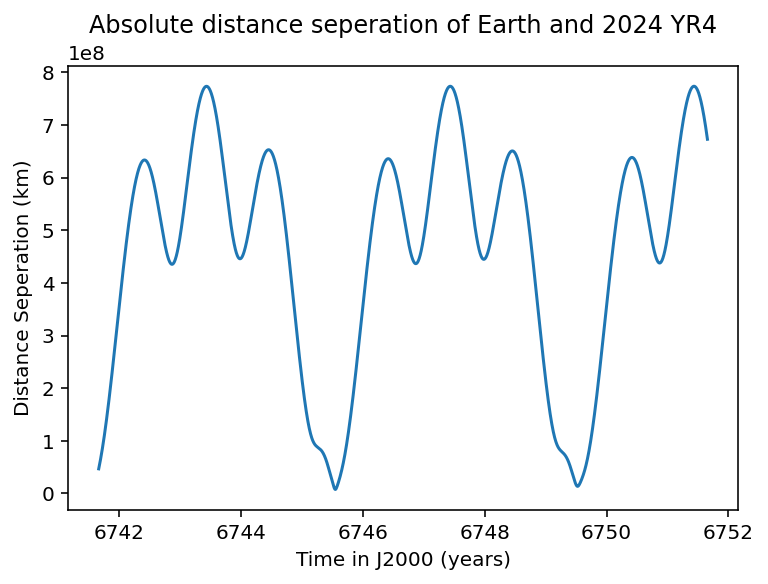
\includegraphics[width=0.48\textwidth]{Images/115-dis.png}
    \caption{Distance between Earth and 2024 YR4 asteroid in kilometers}
\end{figure}

\noindent We can see how the distance is sinusoidal in nature and repeats in an oscillatory fashion. 
This graph shows three distinct peaks, where the middle one is the greatest. We can examine the sydonic period of 
the two bides by examing the equation of the two periods $\frac{1}{T_{syd}} = |\frac{1}{T_{Earth}} - \frac{1}{T_{Asteroid}}|$. And using the orbital periods,
we can see that roughly every 1.33 years, the two bodies are at their closest approach. This lines up well with the graph produced,
showing the magnitude in their seperation. 


\subsection{Numerical Integration}
To derive the necessary state function we have:
\setcounter{equation}{0}
\begin{equation}
    \ddot{\mathbf{r}} = -\frac{\mu}{r^3} \mathbf{r}
\end{equation}
From here we know that $\frac{dv}{dt} = \dot{r}$ giving:
\begin{equation}
    \frac{d\mathbf{v}}{dt} = -\frac{\mu}{r^3} \mathbf{r}
\end{equation}
Expanding each vector as three-dimensional components in $x,y,z$:

\begin{equation}
    \frac{dx}{dt} = v_{x},  \frac{dy}{dt} = v_{y},   \frac{dz}{dt} = v_{z}
\end{equation}


\begin{equation}
    \frac{dv_{x}}{dt} = -\frac{\mu}{r^3} x, \frac{dv_{y}}{dt} = -\frac{\mu}{r^3} y, \frac{dv_{z}}{dt} = -\frac{\mu}{r^3} z
\end{equation}
Where $r = \sqrt{x^{2} + y^{2} + z^{2}}$
\newline
We can now define a state vector $\mathbf{\bar{X}}$


\begin{equation}
    \mathbf{\bar{X}} = 
    \begin{bmatrix}
        x \\
        y \\
        z \\
        v_x \\
        v_y \\
        v_z
        \end{bmatrix}
\end{equation}

Finally, deriving this state vector gives the following:

\begin{equation}
    \mathbf{\dot{\bar{X}}} = 
    \begin{bmatrix}
        v_x \\
        v_y \\
        v_z \\
        -\frac{\mu}{r^3} x \\
        -\frac{\mu}{r^3} y \\
        -\frac{\mu}{r^3} z
        \end{bmatrix}
\end{equation}
Now we can use a function to define the right-hand side of this equation
\begin{lstlisting}
def TBP_ECI(t, state_X, mu):
    x, y, z, vx, vy, vz = state_X  # Unpack state vector
    r = np.sqrt(x**2 + y**2 + z**2)  # Compute radius
    ax, ay, az = -mu * x / r**3, -mu * y / r**3, -mu * z / r**3  # Acceleration components
    return [vx, vy, vz, ax, ay, az]  # Return derivatives
\end{lstlisting}
With this function we can use $SciPy's$ integration feature with solve\_ivp. We can pass 
through a set of initial conditions: a position and velocity vector. It passes through the 
gravitational parameter, $\mu$ as an argument when solving the differential system. Furthermore, 
it uses the Runge-Kutta 45 method to integrate. 
\begin{lstlisting}
r0 = np.linalg.norm(X0[:3])  # Initial distance from Earth's center (km)
v0 = np.linalg.norm(X0[3:])  # Initial speed (km/s)
a = 1/(2/r0 - v0**2/mu_earth)  # Semi-major axis (km)
T = 2 * np.pi * np.sqrt(a**3/mu_earth)  # Orbital period (s)

# Set integration time span for two orbital periods
t_start = 0
t_end = 2 * T  # Two orbital periods
time_step = 10  # Output every 10 seconds
t_eval = np.arange(t_start, t_end, time_step)  

# Solve the system using solve_ivp with strict tolerances
solution = solve_ivp(
    TBP_ECI, (t_start, t_end), X0, t_eval=t_eval, method='RK45',
    args=(mu_earth,), rtol=1e-12, atol=1e-12
)

# Extract components
x, y, z = solution.y[0], solution.y[1], solution.y[2]
vx, vy, vz = solution.y[3], solution.y[4], solution.y[5]
\end{lstlisting}

Using an intital condition, $\bar{X_0}$, we can extrapolate the orbital path. Here, at time zero let 

\begin{equation}
    \mathbf{\bar{X}} = 
    \begin{bmatrix}
        4604.49276873138 \\
        1150.81472538679 \\
        4694.55079634563 \\
        -5.10903235110107   \\
        -2.48824074138143 \\
        5.62098648967432
        \end{bmatrix}
\end{equation}

And the following graph shows the orbital path. I have plotted where the orbit goes behind the Earth with a dashed line,
to express the 3-D nature of this plot, and to also show how this orbit has a very high inclination passing near the North Pole.
\begin{figure}[H]
    \centering
    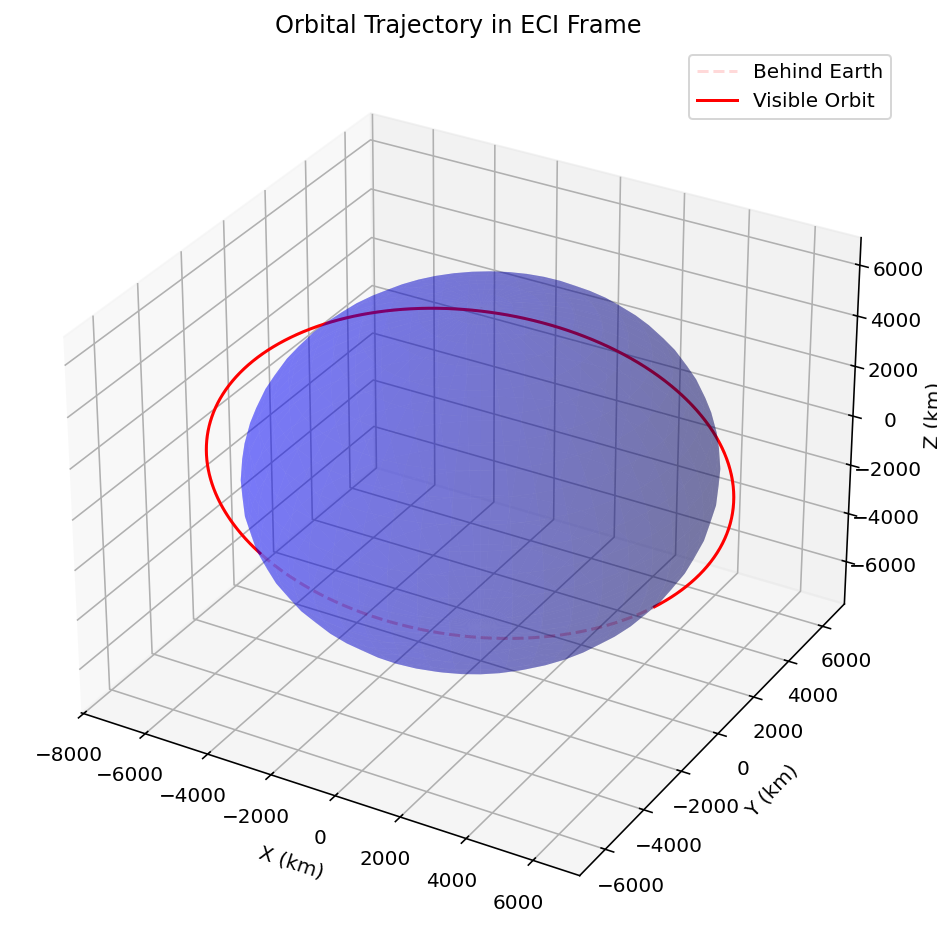
\includegraphics[width=0.48\textwidth]{Images/123-3d.png}
    \caption{Orbital trajectory in ECI frame with initial conditions given from $X_0$}
\end{figure}

Next, we can calculate the how the energies and angular momentum change over time. For each time-step, we can find these values using the following simple orbital equations
\setcounter{equation}{0}
\begin{equation}
E_{k} = \frac{1}{2} \cdot |\bar{v}|^{2}
\end{equation}

\begin{equation}
E_{p} = \frac{-\mu_{earth}}{|\bar{r}|}
\end{equation}

\begin{equation}
\bar{h} = \bar{r} \cross \bar{v}
\end{equation}

By graphing the magnitude of these quantities over time, we can see how the dynamics of this system
\vspace{0.2cm}
\begin{figure}[H]
    \centering
    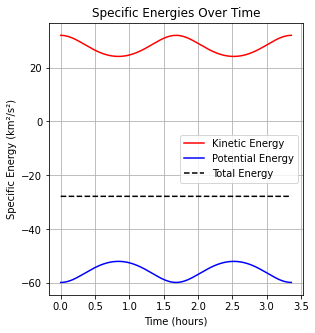
\includegraphics[width=0.4\textwidth]{Images/124-energies.png}
    \caption{How Kinetic, Potential, and Total energies change throughout the orbit }
\end{figure}

This graph shows the sinusoidal nature of the different specific energies. Importantly, we can see how the 
kinetic and potential energies always sum to the same value. This ensures that the total energy remains constant, which we would expect 
as this is a closed system with no external forces. 

\begin{figure}[H]
    \centering
    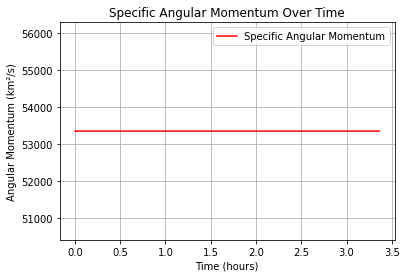
\includegraphics[width=0.48\textwidth]{Images/124-L.png}
    \caption{Graph shows the change in the angular momentum over the orbit is zero}
\end{figure}
\noindent Here, we see this graph depicting how the angular momentum changes over time. It shows how the angular momentum stays 
at a constant value and remains constant. This makes sense because the angular momentum is defined as the cross product
between the position and velocity vector.
\setcounter{equation}{0}
\begin{equation}
\frac{dh}{dt} = \frac{d}{dt}(\bar{r} \times \dot{\bar{r}}) \implies \frac{dh}{dt} = \bar{r} \times \frac{d\dot{\bar{r}}}{dt}
\end{equation}

\begin{equation}
\frac{dh}{dt} = \bar{r} \times -\frac{\mu}{r^{3}}\bar{r} \implies \frac{dh}{dt} = 0
\end{equation}
\vspace{0.2cm}

So yes, these diagrams make physical sense, based upon the conservation laws of both Energy and Angular Momentum


\section{Orbital maneuvers and mission design}
\subsection{Reachability Analysis}
Below defines a function that converts from the state vector containing the position and velocity vector in a 6 x 1 column
to an array containing the six classical orbital elements at that point.

It is important to be in the right quadrant for specific values like $\Omega$, $\omega$, and $\theta$. To ensure this, I have used if statements
to correctly identify when and how these values should be dealt with in order to coincide with convention.
\begin{lstlisting}
def RV2COE(state_x, mu):
    r_vec = state_x[0:3]
    v_vec = state_x[3:6]
    r_mag = norm(r_vec)
    v_mag = norm(v_vec)
    
    a = r_mag / (2 - (r_mag*v_mag**2/mu))
    h = np.cross(r_vec, v_vec)
    h_mag = norm(h)
    e_vec = np.cross(v_vec, h) / mu - r_vec / r_mag
    e_mag = norm(e_vec)
    i = np.arccos(h[2]/h_mag)
    
    n_vec = np.cross(k_hat, h)
    n_mag = norm(n_vec)
    n_hat = n_vec / n_mag
    Omega_raan = np.arccos(n_hat[0])
    if n_hat[1] < 0:
        Omega_raan = 2*np.pi - Omega_raan
    
    omega = np.arccos(np.dot(n_vec, e_vec)/(n_mag * e_mag))
    if e_vec[2] < 0:
        omega = 2*np.pi - omega
        
    cos_theta = np.dot(r_vec, e_vec) / (r_mag * e_mag)
    cos_theta = np.clip(cos_theta, -1.0, 1.0)  
    theta = np.arccos(cos_theta)
    if np.dot(r_vec, v_vec) < 0:
        theta = 2*np.pi - theta
    
    return np.array([a, e_mag, i, Omega_raan, omega, theta])
\end{lstlisting}

Using this function, we can report the COE state for the initial condition. Inputting the vector $\bar{X}$, returns the following elements.

\begin{center}
    \textbf{At } $X_0$:
    COE =
    $\begin{bmatrix}
    a = 7.17813700\mathrm{e}{+03} \\
    e =  7.00000000\mathrm{e}{-02} \\
    i = 1.67551608\mathrm{e}{+00} \\
    \Omega = 3.49065850\mathrm{e}{-01} \\
    \omega = 7.85398163\mathrm{e}{-01} \\
    \theta = 6.28318529\mathrm{e}{+00}
    \end{bmatrix}$  
\end{center}

Next, we can define a rotation matrix that converts from the radius-transverse-normal frame to the ECI frame.
As an input it takes the state vector and outputs a rotation matrix that can be used as an operator.
\begin{lstlisting}
def rotate_matrix(state_x):
    r_vec = state_x[0:3]
    v_vec = state_x[3:6]
    
    r_hat = r_vec/(norm(r_vec))
    

    h_vec = np.cross(r_vec, v_vec)
    h_hat = h_vec / np.linalg.norm(h_vec)  
    t_hat = np.cross(h_hat, r_hat)  

    rotation = np.column_stack((r_hat, t_hat, h_hat))
    
    return rotation
\end{lstlisting}

With this rotation matrix now defined at every point along the orbit, I can define a function named "impulse". This function
takes a rotation matrix, direciton and an initial state as input parameters. It calculates the impulse in the direction of either, 
radius, transverse or normal (which are calculated via 3-D basis vectors). Then the rotation matrix is applied to the impulse to convert
it from the RTN frame to the ECI frame. It adds this vector to the velocity components of the state and then calculates the orbital 
elements of this final state and the inputted initial state to find the difference between components. 
\begin{lstlisting}
def impulse(r_matrix, direct, initial_state):
    dv_ = np.dot(delta_v, direct)

    impulse_eci =  r_matrix @ dv_

    state_final = initial_state.copy()
    state_final[3:] += impulse_eci
    oElements_initial = RV2COE(initial_state, mu_earth)
    oElements_final = RV2COE(state_final, mu_earth)

    coe_diff = oElements_final - oElements_initial

    return coe_diff, oElements_final
\end{lstlisting}

Using these combinations of functions we can apply an impulse in the three different directions and calculate the changes.
\begin{table}[h]
    \centering
    \begin{minipage}{0.48\textwidth} % First table: first three columns
        \centering
        \small
        \setlength{\tabcolsep}{4pt}
        \renewcommand{\arraystretch}{1.1}
        \begin{tabular}{lccc}
        \hline
        Impulse Type & $\Delta a$ & $\Delta e$ & $\Delta i$ \\
        \hline
        Radial     & 0.012927 & $1.28\mathrm{e}{-5}$ & 0 \\
        Transverse & 20.7374  & 0.00267900   & 0 \\
        Normal     & 0.012927 & $1.67\mathrm{e}{-6}$ & $8.85\mathrm{e}{-4}$ \\
        \hline
        \end{tabular}
        \caption{Changes in the semi-major axis, eccentricity and inclination}
    \end{minipage}
    \hfill
    \begin{minipage}{0.48\textwidth} % Second table: last three columns
        \centering
        \small
        \setlength{\tabcolsep}{4pt}
        \renewcommand{\arraystretch}{1.1}
        \begin{tabular}{ccc}
        \hline
        $\Delta \Omega$ & $\Delta \omega$ & $\Delta M$ \\
        \hline
        0 & -0.0191214 & -6.26406 \\
        0 & 0 & 0.0000000149012 \\
        0.000889606 & 0.0000933805 & 0.0000000149012 \\
        \hline
        \end{tabular}
        \caption{Changes in $\Omega$, $\omega$ and mean anamoly}
    \end{minipage}
\end{table}

    

    \begin{figure}[H]
        \centering
    
        % First row
        \begin{subfigure}[t]{0.45\textwidth}
            \centering
            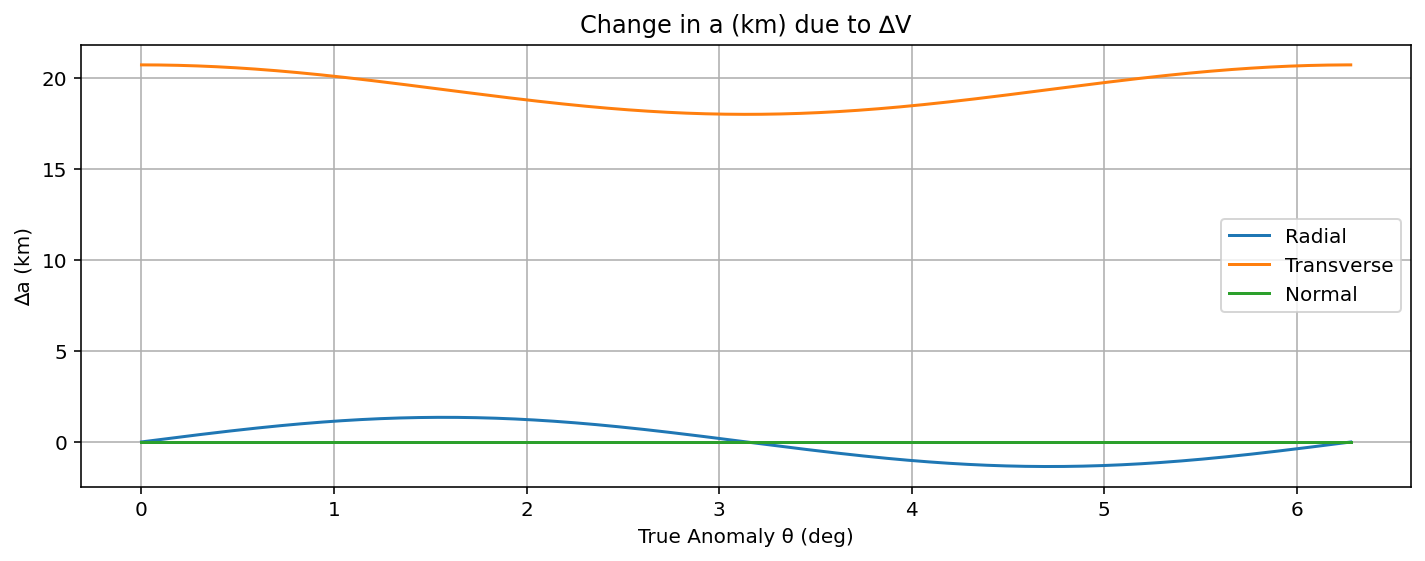
\includegraphics[width=\linewidth]{Images/del_a.png}
            \caption{Graph 1}
        \end{subfigure}
        \hspace{0.05\textwidth}
        \begin{subfigure}[t]{0.45\textwidth}
            \centering
            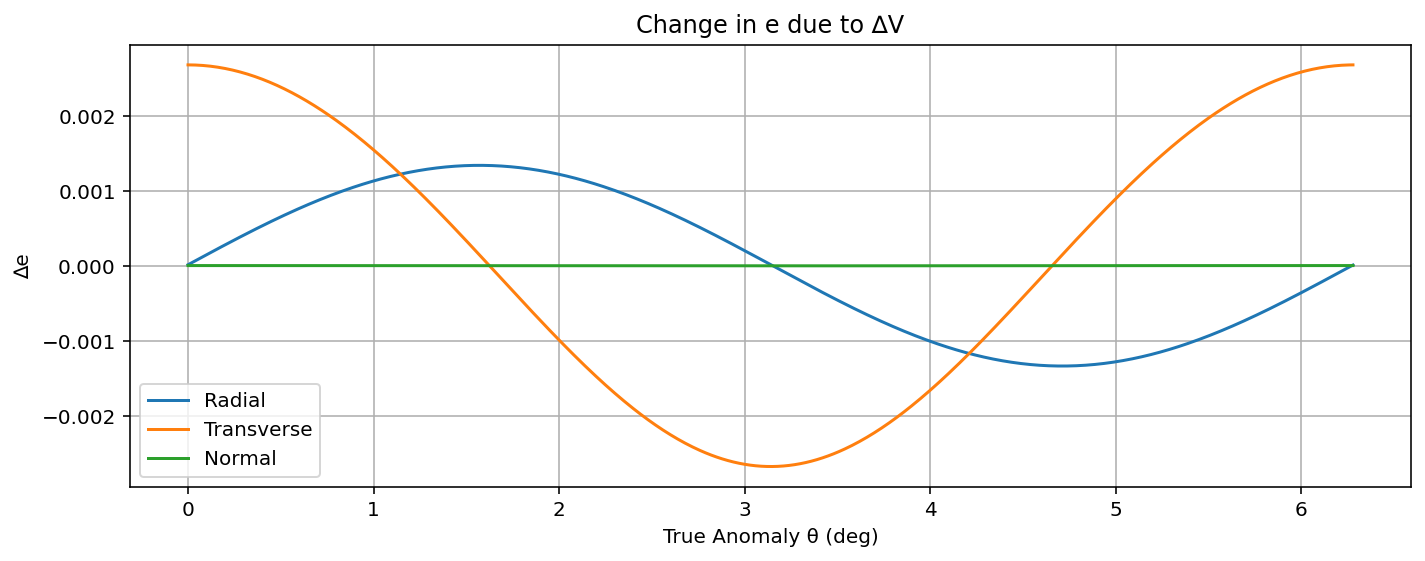
\includegraphics[width=\linewidth]{Images/del_e.png}
            \caption{Graph 2}

        \end{subfigure}
    
        \vspace{1em}
    
        % Second row
        \begin{subfigure}[t]{0.45\textwidth}
            \centering
            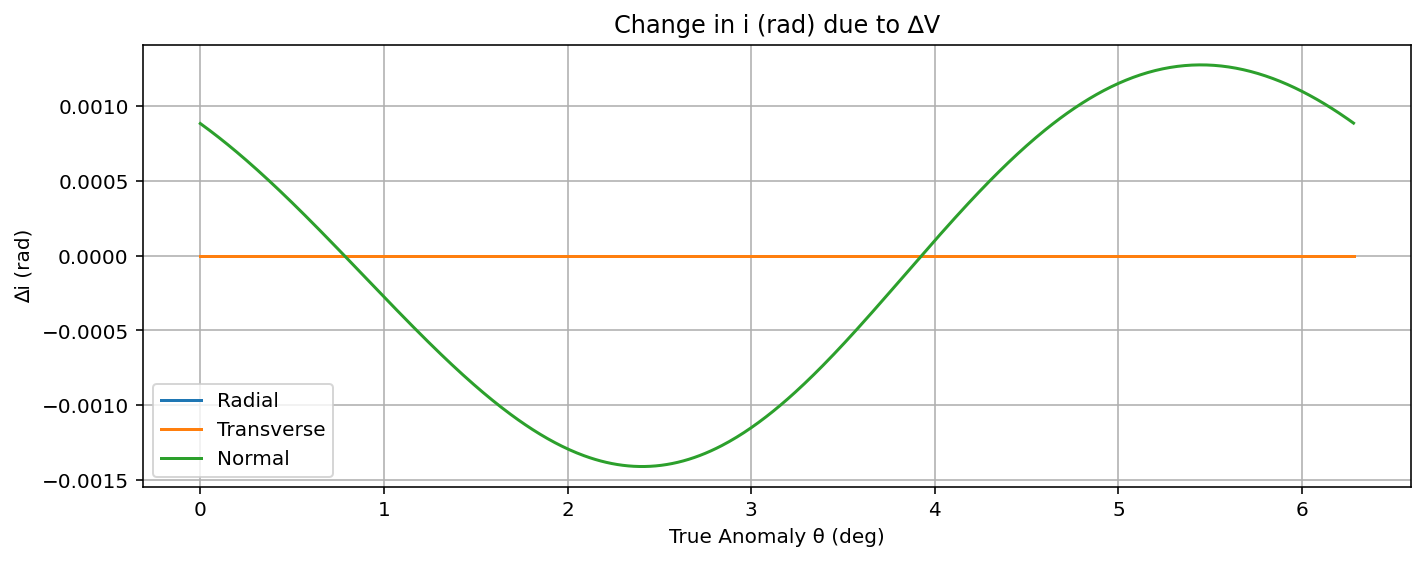
\includegraphics[width=\linewidth]{Images/del_i.png}
            \caption{Graph 3}
        \end{subfigure}
        \hspace{0.05\textwidth}
        \begin{subfigure}[t]{0.45\textwidth}
            \centering
            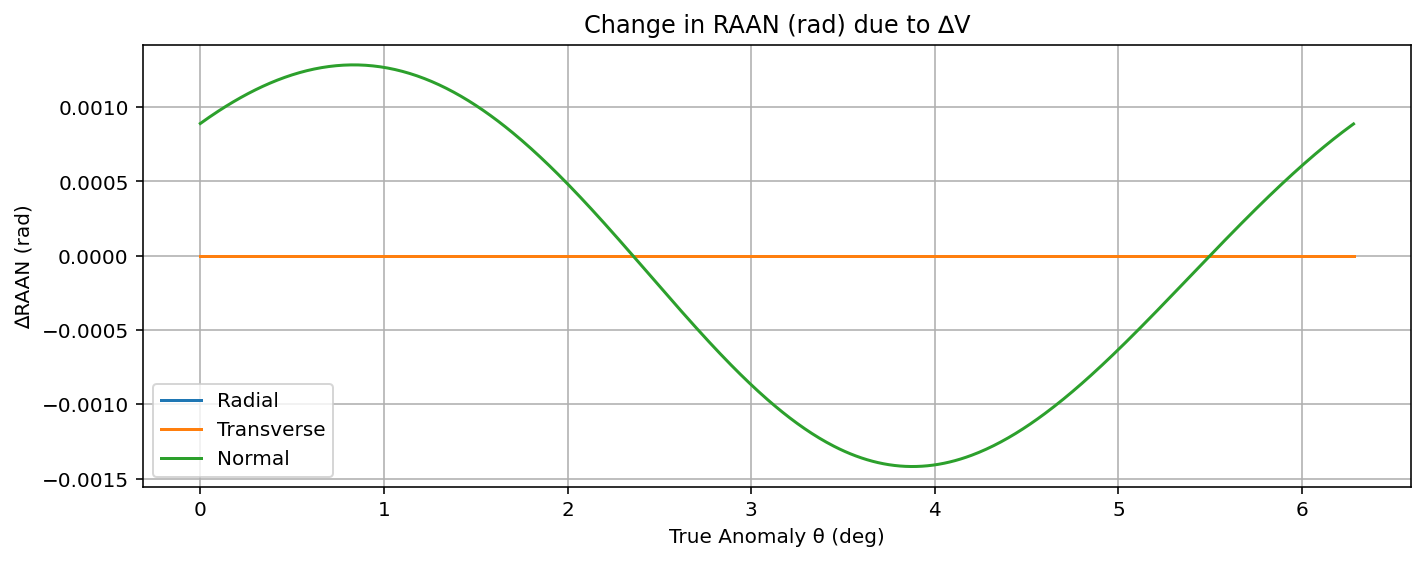
\includegraphics[width=\linewidth]{Images/del_Omega.png}
            \caption{Graph 4}
        \end{subfigure}
    
        \vspace{1em}
    
        % Third row
        \begin{subfigure}[t]{0.45\textwidth}
            \centering
            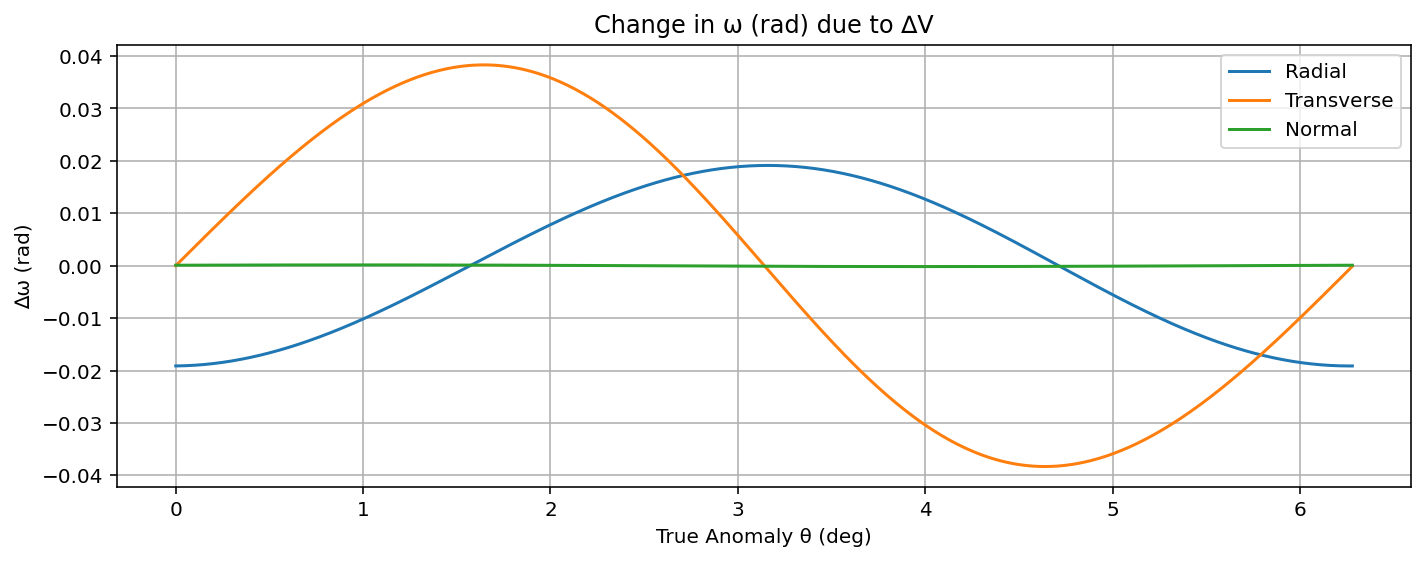
\includegraphics[width=\linewidth]{Images/del_lomega.png}
            \caption{Graph 5}
        \end{subfigure}
        \hspace{0.05\textwidth}
        \begin{subfigure}[t]{0.45\textwidth}
            \centering
            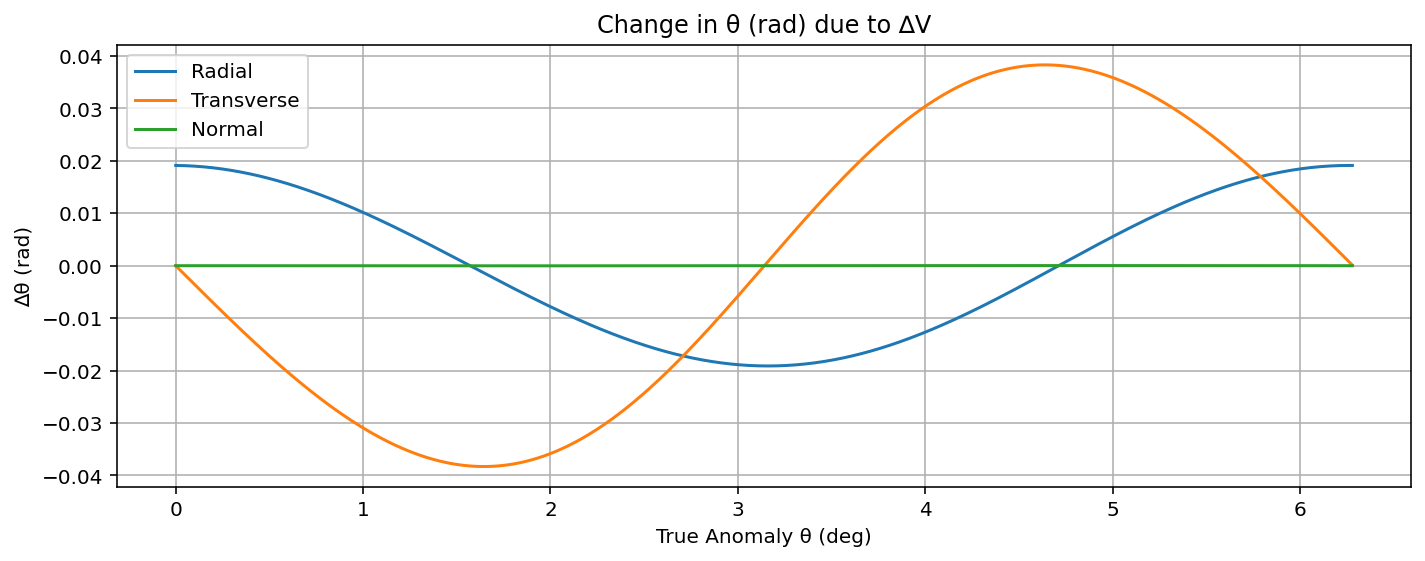
\includegraphics[width=\linewidth]{Images/del_theta.png}
            \caption{Graph 6}
        \end{subfigure}
    
        \caption{Six graphs showing how the classical orbital elements change with impulses}
        \label{fig:six_graphs}
    \end{figure}
Using these graphs we can examine which $\theta$ values maximise $\Delta i$. Using the Signal library apart of Python
and its corrosponding find\_peaks\_cwt function, the peaks of $\Delta i$ are  $-0.0014$ and $0.0013$ radians.
These corrosponding $\theta$ values are $2.36$ and $5.46$ radians. Understanding that the argument of latitude, $u$,
is defined as $\theta + \omega$, and observing that at these theta values, $\omega = 0.79$ and $0.79$ radians.
Hence, $u = 3.145$ and $6.245$ radians. These numbers represent the apogee and perigee respectively (which make sense because the perigee and apogee 
occur at $\pi$ and $2\pi$). Therefore, for maximum change to the inclination, one should provide a normal impulse at the perigee and apogee.

\subsection{Lunar Mission Design}

\noindent Now we can analyse what happens when the apogee of the transfer orbit is increased passed the 
orbital radius of the moon. By increasing this distance 
we are completeing a non-tangential transfer, where the mission will have a lower transfer time, but will arrive
with some non-zero radial velocity.

Using numpy's matrix-oriented math in Python, calculations can be swift looking at the range of 
apogee values. The following code uses the range of apogee values to calculate the semi-major axis, eccentricity, the true anamoly, and the semi-latus rectum,
to ultimately return the radial and transverse components of the arrival velocity vector. 
\begin{lstlisting}
parking_altitude = 220
r_p = parking_altitude + radius_earth

r_a = r_mean*np.arange(1.1, 1.4, 0.01)
a = 0.5*(r_p + r_a)
ecc = (r_a-r_p)/(r_a+r_p)
cos_theta_A = (a * (1 - ecc**2) / r_mean - 1) / ecc
theta_2 = np.arccos(cos_theta_A)
p =  a * (1 - ecc**2)

v_radial = np.sqrt(mu_earth / p) * ecc * np.sin(theta_2)
v_transverse = np.sqrt(mu_earth / p) * (1 + ecc * np.cos(theta_2))
normed_apogee = r_a/r_mean
\end{lstlisting} 

\noindent Now we have the true anamoly, radial, and transverse velocities inside a matrix array for every 
apogee value normalized to the moon's orbital radius. Printing these components, we can see how 
these change as we increase the distance. 
\begin{figure}[H]
    \centering
    \begin{minipage}{0.48\textwidth}
        \centering
        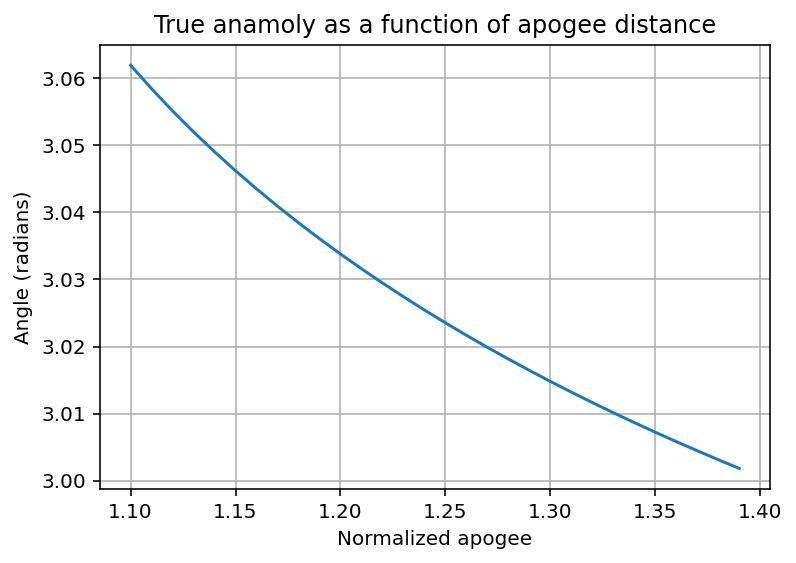
\includegraphics[width=\textwidth]{Images/221-theta.png}
        \caption{Graph depicting how the true anamoly decreases as the apogee distance increases}

    \end{minipage}
    \hfill
    \begin{minipage}{0.48\textwidth}
        \centering
        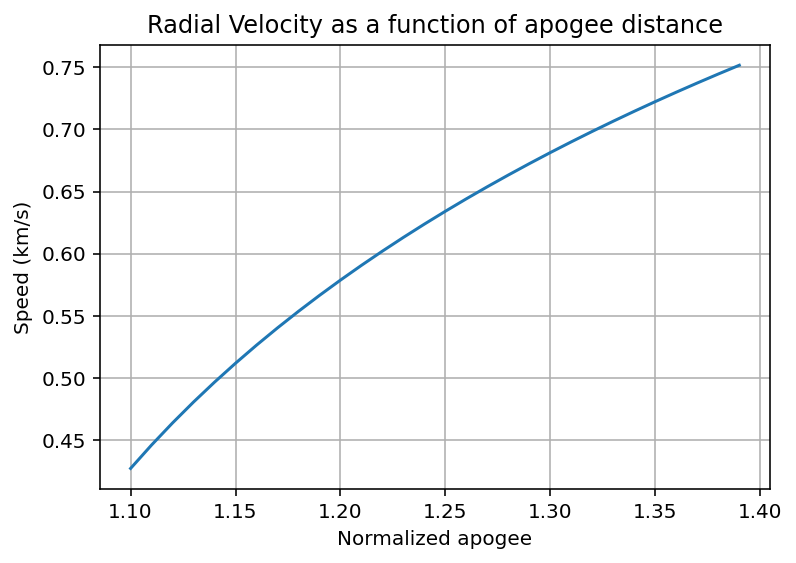
\includegraphics[width=\textwidth]{Images/221-rad.png}
        \caption{Graph depicting how the radial velocity increases as the apogee distance increases}

    \end{minipage}
    \hfill
    \begin{minipage}{0.48\textwidth}
        \centering
        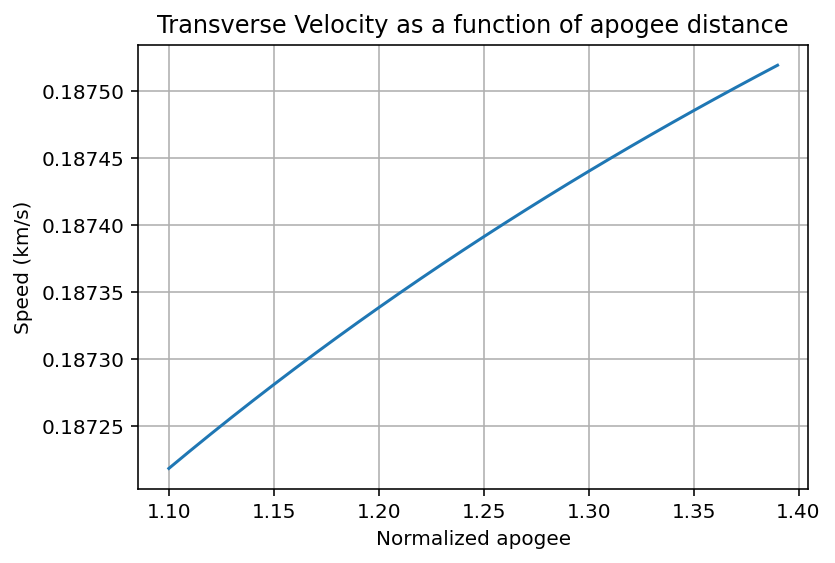
\includegraphics[width=\textwidth]{Images/221-trans.png}
        \caption{Graph depicting how the transverse velocity increases as the apogee distance increases}
    \end{minipage}
\end{figure}
The first plot shows how the true anamoly decreases with apogee. This means that the spacecraft
is intercepting the moon at an earlier point along its orbit. At an normalized apogee of 1, this represents
a Hohman transfer so its true anamoly would be $\pi$, as we increase the apogee distance, this angle decreases.
\vspace{0.75cm}
\newline
We can also see from these figures how the radial component of the velocity 
changes much more significantly that the transverse component.
This is because the radial component is related
 to the orbital energy equation. When the 
semi-major axis is significantly increased, 
to reach beyond the Moon, most of that additional energy 
manifests as radial velocity because it 
directly contributes to increasing the orbital energy and apogee height.
By comparison, the transverse velocity is primarily responsible 
for maintaining orbital angular momentum, so does not change as violently.
\vspace{0.75cm}
\newline
Next we can observe how the apogee and transfer time are related.
Writing some more code we can examine this, again using numpy's matrix operations.
\begin{lstlisting}
theta_eccentric = 2*np.arctan(np.tan(theta_2/2) * ((1-transfer_e)/(1+transfer_e))**(0.5))
theta_mean = theta_eccentric - transfer_e*np.sin(theta_eccentric)
time_total = time_orbit(semi_major_axis, mu_earth)
delta_t = (time_total / (2 * np.pi)) * theta_mean / days_convert
\end{lstlisting}
This gives the transfer time for every apogee value, which we can plot as the following.

\begin{figure}[H]
    \centering
    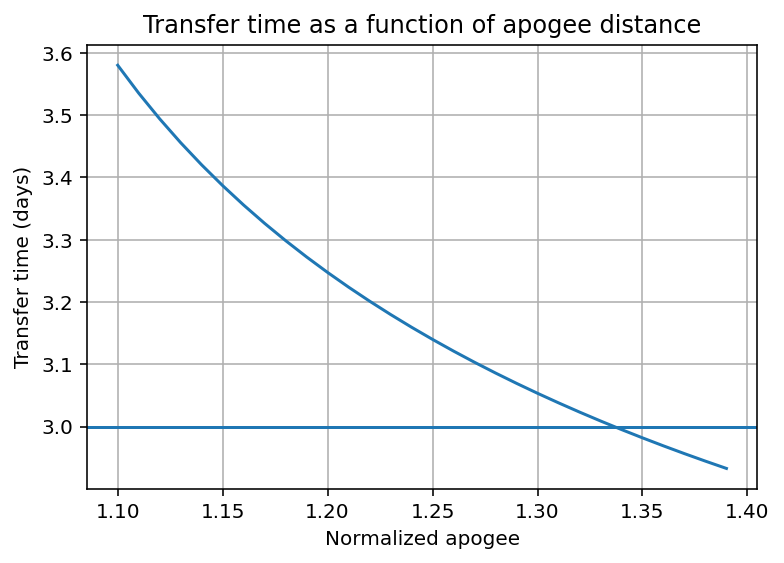
\includegraphics[width=0.48\textwidth]{Images/222-time.png}
    \caption{Graph showing how the transfer time decreases as the apogee value increases}
\end{figure}

This plot clearly shows how the transfer time decreases as the apogee value increases. This makes sense because increasing the 
apogee point, means the spacecraft is intercepting the moon at an earlier stage of its orbit.
There is a horizontal line corrosponding to $t=3$ days. We can look at the intercept of this line with the plot to see that for a 
transfer time of three days, an apogee value of $1.34\cdot r_m$ is required.
\vspace{0.75cm}
\newline
Finally, we can compare the transfer time with the minimum required perilune altitude for a free return back to Earth.
Assuming the moon is moving in a circular orbit, this implies that it only has velocity components in the transverse direction.
The following script uses this idea to calculate the hyperbolic quantities for a free return trajectory, ultimately returning the 
minimum required perilune altitude.
\begin{lstlisting}
    v_moon = np.sqrt(mu_earth/r_mean)

    v_ir = v_radial
    v_it = v_transverse-v_moon
    v_infminus = np.sqrt(v_radial**2 + v_it**2)
    
    quotient = -v_ir / v_it
    delta_angle = np.arctan(quotient)
    hyperbolic_e = (np.sin(delta_angle))**-1
    r_perilune = (hyperbolic_e - 1)*mu_moon/(v_infminus**2)
    altitude_perilune = r_perilune - radius_moon
\end{lstlisting}
\begin{figure}[H]
    \centering
    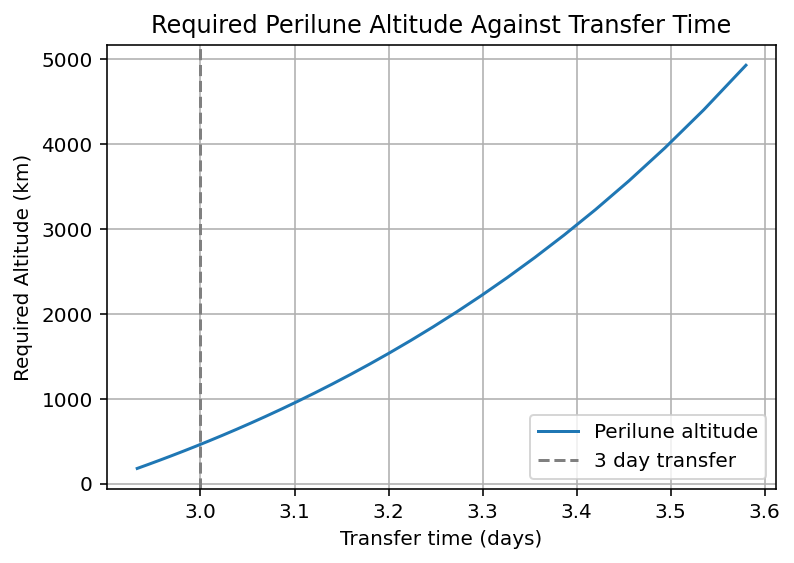
\includegraphics[width=0.48\textwidth]{Images/223-altitude.png}
    \caption{Distance between Earth and 2024 YR4 asteroid in kilometers}
\end{figure}

This plot shows how for a three day transfer, the minimum required perilun altitude is \textbf{insert here}. This lines up 
closesly with the Apollo 11 mission, where the Wiki states "The craft passes on the near side of the Moon at a radius of 2150 km (410 km above the surface) and is thrown back outwards."
\begin{adjustwidth}{-0.5cm}{0cm}

    \begin{tikzpicture}[scale=1.5]
    
      \draw[->] (0,0) -- (2*-2.5,0)node[anchor=north east, font=\tiny]{$v_{\theta}$};
      \draw[->] (0,2*-1) -- (0,2*1)node[anchor=north west, font=\tiny]{$v_{r}$};
    
      \draw[->,red] (0,0) -- (0,2*0.71);
      \draw[->,blue] (0,0) -- (-4*0.18,0);

      \draw[dashed] (-4*0.18,2*-1) -- (-4*0.18,2*1);
      \draw[dashed] (-4*0.18,2*0.71) -- (0,2*0.71);
    
      \draw[->,green] (0,0) -- (-4*0.18,2*0.71);
      \draw[->,green] (0,0) -- (-4*0.18,2*-0.71);
    
      \node at (2*-2,0) {$+$};
      \node[xshift= -6cm, yshift= -0.35cm, font=\tiny]{$v_{\leftmoon}$};
      
      \draw[->,purple] (2*-2,0) -- (-4*0.18,2*0.71) node[xshift= -2cm, yshift= -0.35cm, font=\tiny]{$v_{\infty}^{-}$};
      \draw[->,purple] (2*-2,0) -- (-4*0.18,2*-0.71) node[xshift= -2cm, yshift= 0.35cm, font=\tiny]{$v_{\infty}^{+}$}; 
    
    
      \coordinate (A) at (-2,0.9);
      \coordinate (B) at (2*-2,0);
      \coordinate (C) at (-2,0);
      \pic[draw,-,black,angle radius=1cm] {angle = C--B--A};
      \node[xshift= 1.5cm, yshift= 0.2cm, font=\tiny] at (B) {$ \delta$=81.4\textdegree.};
    
    
    \end{tikzpicture}

\end{adjustwidth}

This diagram represents the free return 
symmetric trajectory representative of a 
required perilune altitude of \textbf{insert here}

\onecolumn
\section{Appendix}
   
\begin{minted}{python}
    # -*- coding: utf-8 -*-
"""
Created on Tue Mar 25 22:08:35 2025

@author: alexa
"""



#Import Python files
import matplotlib.pyplot as plt
import numpy as np
from mpl_toolkits.mplot3d import Axes3D
from scipy.integrate import solve_ivp
from scipy import signal

show_plots = False



#Assignment Data

mu_sun = 1.3271244*10**11
mu_earth = 3.986*10**5
radius_earth = 6378.14
J_2_earth = 1082.63*10**-6
mu_moon = 4902.8
radius_moon = 1737.4
r_mean = 384400


'''
Functions
'''

def norm(vec):
    return np.linalg.norm(vec)

pi = np.pi
def radians(deg):
    rads = deg * (pi/180)
    return rads


def get_mean_anamoly(del_t, M_old, a):
    nu_t = (mu_sun / (a**3))**0.5
    mean_anamoly_t = M_old + nu_t * (del_t)
    
    return mean_anamoly_t

def time_orbit(a, μ):
    T = 2 * np.pi * np.sqrt(a**3 / μ)
    time = T 
    return time

def rotation_matrix(i, Omega, omega):
    cos_O, sin_O = np.cos(Omega), np.sin(Omega)
    cos_i, sin_i = np.cos(i), np.sin(i)
    cos_w, sin_w = np.cos(omega), np.sin(omega)
    
    R = np.array([
        [cos_O * cos_w - sin_O * sin_w * cos_i, -cos_O * sin_w - sin_O * cos_w * cos_i, sin_O * sin_i],
        [sin_O * cos_w + cos_O * sin_w * cos_i, -sin_O * sin_w + cos_O * cos_w * cos_i, -cos_O * sin_i],
        [sin_w * sin_i, cos_w * sin_i, cos_i]
    ])
    
    return R

'''
Newton-Rasphon Method to return the eccentric anamoly to a certain tolerance
'''

#1.1.1 ----------------------------------------------------------------------


def Kepler(e, M, tol = 1e-12, max_i = 1000):
    E = M
    
    
    for i in range(max_i):
        
        f_E = E - e * np.sin(E) - M
        f_prime = 1 - e * np.cos(E)
        
        del_E = f_E / f_prime
        
        
        E_new = E - del_E
        if np.abs(del_E) < tol:
            theta = 2*np.arctan(np.tan(E_new/2) * ((1+e)/(1-e))**(0.5))
            return theta
        E = E_new
 
        



    
E_ae0 = [2460705.5, 1.495988209443421E+08, 1.669829008180246E-02, radians(3.248050135173038E-03), 
          radians(1.744712892867145E+02), radians(2.884490093009512E+02), radians(2.621190445180298E+01)]


A_ae0 = [2460705.5, 3.764419202360106E+08, 6.616071771587672E-01, radians(3.408286057191753),
          radians(2.713674649188756E+02), radians(1.343644678984687E+02), radians(1.693237490356061E+01)]



#1.1.2 ----------------------------------------------------------------------


trueAnamoly_asteroidt_0 = Kepler(A_ae0[2], A_ae0[6])
meanAnamolyt_100 = get_mean_anamoly(100*(3600*24), A_ae0[6], A_ae0[1])
trueAnamoly_asteroidt_100 = Kepler(A_ae0[2], meanAnamolyt_100)

# print(trueAnamoly_asteroidt_0)
# print(trueAnamoly_asteroidt_100)



Obj2_t0 = A_ae0.copy()
Obj2_t0[6] = trueAnamoly_asteroidt_0
Obj2_t0 = Obj2_t0[1:]


Obj2_t100 = A_ae0.copy()
Obj2_t100[6] = trueAnamoly_asteroidt_100
Obj2_t100 = Obj2_t100[1:]

#1.1.3 ----------------------------------------------------------------------

t_0 = 2460705.5*(3600*24)

def COE2RV(arr, mu):
    a, e, i, Omega, omega, theta_var = arr[0:6]
    h = np.sqrt(mu * a * (1 - e**2))
    r = a*(1-(e**2))/(1 + e*np.cos(theta_var))
    
    arr_r = np.array([r*np.cos(theta_var), r*np.sin(theta_var), 0])
    arr_v = (mu/h)* np.array([-np.sin(theta_var), e + np.cos(theta_var), 0])

    #Rotate position and velocity from perifocal to inertial frame using the transfomration matrix
    R_matrix = rotation_matrix(i, Omega, omega)
   
    r_ijk = R_matrix @ arr_r
    v_ijk = R_matrix @ arr_v
    return r_ijk, v_ijk




state_vector_0 = np.array(COE2RV(Obj2_t0, mu_sun))
#print(state_vector_0) # t = t0



state_vector_100 = np.array(COE2RV(Obj2_t100, mu_sun))
#print(state_vector_100) # t = t0 + 100

# print('\n')
# print(state_vector_0 - state_vector_100)

t_0_days = 2460705.5
days_convert = 3600*24
#1.1.4 ----------------------------------------------------------------------

def Ephemeris(t, OBJdata, mu):

    time, a, e, i, Omega, omega, mean_anamoly = OBJdata[0:7]
    nu_t = (mu / (a**3))**0.5
    
    t = t - t_0_days*days_convert
    mean_anamoly_t = mean_anamoly + nu_t * (t)

    h = np.sqrt(mu * a * (1 - e**2))
    
    theta_var = Kepler(e, mean_anamoly_t)
    r = a*(1-(e**2))/(1 + e*np.cos(theta_var))
    
    arr_r = np.array([r*np.cos(theta_var), r*np.sin(theta_var), 0])
    arr_v = (mu/h)* np.array([-np.sin(theta_var), e + np.cos(theta_var), 0])
    
    R_matrix = rotation_matrix(i, Omega, omega)
    r_ijk = R_matrix @ arr_r
    v_ijk = R_matrix @ arr_v
    
    return r_ijk, v_ijk




years_shown_i = 1
t_array = days_convert*np.arange(t_0_days,t_0_days+years_shown_i*365, 1) 

x_earth = np.zeros((6,len(t_array)))
x_asteroid = np.zeros((6,len(t_array)))

 
for r in range(len(t_array)):
    x_earth[0:6, r] = np.hstack(Ephemeris(t_array[r], E_ae0, mu_sun))
    x_asteroid[0:6, r] = np.hstack(Ephemeris(t_array[r], A_ae0, mu_sun))
    

t_day_array = np.arange(0, years_shown_i*365, 1)
time_Earth = time_orbit(E_ae0[1], mu_sun)/days_convert # Convert from seconds to days
orbital_percent_E = (t_day_array / time_Earth) 


plt.plot(orbital_percent_E,[norm(x_earth[0:3, t]) for t in range(len(t_array))], label="Earth position", color='b')
plt.plot(orbital_percent_E, [norm(x_asteroid[0:3, t]) for t in range(len(t_array))], label="Asteroid position", color='r')
plt.legend()
plt.title("Magnitude of the Position of Earth and 2024 YR4 Asteroid")
plt.xlabel("Percent of Earth's Orbit (%)")
plt.ylabel("Position Vector (km)")
if show_plots:
    plt.show()
else:
    plt.close()

plt.figure()
plt.plot(orbital_percent_E,[norm(x_earth[3:, t]) for t in range(len(t_array))], label="Earth velocity", color='b')
plt.plot(orbital_percent_E, [norm(x_asteroid[3:, t]) for t in range(len(t_array))], label="Asteroid velocity", color='r')
plt.legend()
plt.xlabel("Percent of Earth's Orbit (%)")
plt.ylabel("Velocity Vector (km/s)")
plt.title("Magnitude of the Velocity of Earth and 2024 YR4 Asteroid")

if show_plots:
    plt.show()
else:
    plt.close()
    
years_shown = 10
t_total = days_convert*np.arange(t_0_days, t_0_days + years_shown*365, 1)



normed_diff = []
for t in t_total:
    
    normed_diff.append(norm(Ephemeris(t,E_ae0, mu_sun)[0] - Ephemeris(t,A_ae0, mu_sun)[0]))
    
    
plt.figure()
#plt.plot(t_total*(10/t_total[-1]), normed_diff)
plt.plot(t_total/(days_convert*365), normed_diff)
plt.title("Absolute distance seperation of Earth and 2024 YR4")
plt.xlabel("Time in J2000 (years)")
plt.ylabel("Distance Seperation (km)")
if show_plots:
    plt.show()
else:
    plt.close()

#1.2.1 ----------------------------------------------------------------------

x0, y0, z0 = 4604.49276873138, 1150.81472538679, 4694.55079634563   # km
vx0, vy0, vz0 = -5.10903235110107 , -2.48824074138143 ,5.62098648967432   # km/s

# Pack initial state vector
X0 = [x0, y0, z0, vx0, vy0, vz0]    

#1.2.2 ----------------------------------------------------------------------

def TBP_ECI(t, state_X, mu):
    x, y, z, vx, vy, vz = state_X  # Unpack state vector
    r = np.sqrt(x**2 + y**2 + z**2)  # Compute radius
    ax, ay, az = -mu * x / r**3, -mu * y / r**3, -mu * z / r**3  # Acceleration components
    return [vx, vy, vz, ax, ay, az]  # Return derivatives



#1.2.3 ----------------------------------------------------------------------

r0 = np.linalg.norm(X0[:3])  # Initial distance from Earth's center (km)
v0 = np.linalg.norm(X0[3:])  # Initial speed (km/s)
a = 1 / (2 / r0 - v0**2 / mu_earth)  # Semi-major axis (km)
T = 2 * np.pi * np.sqrt(a**3 / mu_earth)  # Orbital period (s)

# Set integration time span for two orbital periods
t_start = 0
t_end = 2 * T  # Two orbital periods
time_step = 10  # Output every 10 seconds
t_eval = np.arange(t_start, t_end, time_step)  

# Solve the system using solve_ivp with strict tolerances
solution = solve_ivp(
    TBP_ECI, (t_start, t_end), X0, t_eval=t_eval, method='RK45',
    args=(mu_earth,), rtol=1e-12, atol=1e-12
)

# Extract components
x, y, z = solution.y[0], solution.y[1], solution.y[2]
vx, vy, vz = solution.y[3], solution.y[4], solution.y[5]

r = np.sqrt(x**2 + y**2 + z**2)

# Compute speed
v_lin = np.sqrt(vx**2 + vy**2 + vz**2)

# 3D Trajectory Plot
fig = plt.figure(figsize=(8, 8))
ax = fig.add_subplot(111, projection='3d')


#Plot Earth as a sphere
earth_radius = 6378  # km (mean Earth radius)
u, v = np.mgrid[0:2*np.pi:50j, 0:np.pi:25j]
X_earth = earth_radius * np.cos(u) * np.sin(v)
Y_earth = earth_radius * np.sin(u) * np.sin(v)
Z_earth = earth_radius * np.cos(v)
ax.plot_surface(X_earth, Y_earth, Z_earth, color='b', alpha=0.3)


# Plot the orbit
# Dashed section 
ax.plot(x[:460], y[:460], z[:460], color='r', label='Behind Earth',linestyle='dashed', alpha = 0.15)

# Dashed segment (between 460 and 890)
ax.plot(x[460:891], y[460:891], z[460:891], color='r', linewidth=1.5, label='Visible Orbit')

ax.plot(x[891:], y[891:], z[891:], color='r',linestyle='dashed', alpha = 0.15)


# Labels and title
ax.set_xlabel("X (km)")
ax.set_ylabel("Y (km)")
ax.set_zlabel("Z (km)")
ax.set_title("Orbital Trajectory in ECI Frame")
ax.legend()
plt.show()
# if show_plots:
#     plt.show()
# else:
#     plt.close()    
    
    
#1.2.4 ----------------------------------------------------------------------


plt.figure()

KE = 0.5 * v_lin**2
PE = -mu_earth / r
E_total = KE + PE


x, y, z = solution.y[0], solution.y[1], solution.y[2]
vx, vy, vz = solution.y[3], solution.y[4], solution.y[5]
# Compute Specific Angular Momentum (km²/s)
h_array = np.sqrt(((y * vz) - (z * vy))**2 + ((z * vx) - (x * vz))**2 + ((x * vy) - (y * vx))**2)
# Convert time to hours for better readability
time_hours = solution.t / 3600

# Plot Specific Energies
plt.figure(figsize=(10, 5))

plt.subplot(1, 2, 1)
plt.plot(time_hours, KE, label="Kinetic Energy", color='r')
plt.plot(time_hours, PE, label="Potential Energy", color='b')
plt.plot(time_hours, E_total, label="Total Energy", color='k', linestyle='dashed')
plt.xlabel("Time (hours)")
plt.ylabel("Specific Energy (km²/s²)")
plt.title("Specific Energies Over Time")
plt.legend()
plt.grid()

if show_plots:
    plt.show()
else:
    plt.close()

# Plot Specific Angular Momentum
plt.figure()
plt.plot(time_hours, h_array.round(2),'r', label="Specific Angular Momentum")
plt.xlabel("Time (hours)")
plt.ylabel("Angular Momentum (km²/s)")
plt.title("Specific Angular Momentum Over Time")
plt.legend()
plt.grid()

if show_plots:
    plt.show()
else:
    plt.close()
    
    
#2.1.1 ----------------------------------------------------------------------

k_hat = np.array([0,0,1])


def RV2COE(state_x, mu):
    #x,y,z,vx,vy,vz = state_x
    r_vec = state_x[0:3]
    v_vec = state_x[3:6]
    r_mag = norm(r_vec)
    v_mag = norm(v_vec)
    
    a = r_mag / (2 - (r_mag*v_mag**2/mu))
    
    h = np.cross(r_vec, v_vec)
    h_mag = norm(h)
    e_vec = np.cross(v_vec, h) / mu - r_vec / r_mag
    e_mag= np.linalg.norm(e_vec)
    
    i = np.arccos(h[2]/h_mag)
    
    n_vec = np.cross(k_hat, h)
    n_mag = norm(n_vec)
    n_hat = n_vec / n_mag
    Omega_raan = np.arccos(n_hat[0])
    
    if n_hat[1] < 0:
        Omega_raan = 2*np.pi - Omega_raan
    
    
    omega = np.arccos(np.dot(n_vec, e_vec)/(n_mag * e_mag))
    
    if e_vec[2] < 0:
        omega = 2*np.pi - omega
        
    
    cos_theta = np.dot(r_vec, e_vec) / (r_mag * e_mag)
    cos_theta = np.clip(cos_theta, -1.0, 1.0)  # ensures it's in valid domain
    theta = np.arccos(cos_theta)
    
    if np.dot(r_vec, v_vec) < 0:
        theta = 2*np.pi - theta
    
    
    return np.array([a, e_mag, i, Omega_raan, omega, theta])
    
    


#print(RV2COE(X0, mu_earth))
    
#2.1.2 ----------------------------------------------------------------------

def rotate_matrix(state_x):
    r_vec = state_x[0:3]
    v_vec = state_x[3:6]
    
    r_hat = r_vec/(norm(r_vec))
    

    h_vec = np.cross(r_vec, v_vec)
    h_hat = h_vec / np.linalg.norm(h_vec)  # N (Normal) direction
    t_hat = np.cross(h_hat, r_hat)  

    rotation = np.column_stack((r_hat, t_hat, h_hat))
    
    return rotation

#2.1.3 ----------------------------------------------------------------------

delta_v = 0.01
rotation_transform = rotate_matrix(X0)


def impulse(r_matrix, direct, initial_state):
    
    dv_ = np.dot(delta_v, direct)
    
    impulse_eci =  r_matrix @ dv_
    
    state_final = initial_state.copy()
    state_final[3:] += impulse_eci
    oElements_initial = RV2COE(initial_state, mu_earth)
    oElements_final = RV2COE(state_final, mu_earth)
    
    coe_diff = oElements_final - oElements_initial
    
    return coe_diff, oElements_final
    
    

# '''
# Reporting the different states for the radial, transverse and normal impulses at that point
# '''

er = [1,0,0]
et = [0,1,0]
en = [0,0,1]
# print(impulse(rotate_matrix(X0), er, X0)[0])
# print(impulse(rotate_matrix(X0), et, X0)[0])
# print(impulse(rotate_matrix(X0), en, X0)[0])


#2.1.4 ----------------------------------------------------------------------

oElements_initial = RV2COE(X0, mu_earth)
theta_array = np.arange(0,2*np.pi, 0.01)

delta_elements_radial = []
delta_elements_transverse = []
delta_elements_normal = []

all_elements_N = np.zeros((6,len(theta_array)))
i = 0
for theta in theta_array:
    
    coe = oElements_initial.copy()
    coe[5] = theta
    state_RV = np.concatenate(COE2RV(coe, mu_earth))
    
    rotation = rotate_matrix(state_RV)
    
    
    delta_elements_radial.append(impulse(rotation, er, state_RV)[0])
    delta_elements_transverse.append(impulse(rotation, et, state_RV)[0])
    delta_elements_normal.append(impulse(rotation, en, state_RV)[0])
    
    all_elements_N[0:6, i] = impulse(rotation, en, state_RV)[1]
    i = i + 1

deltaR_array = np.array(delta_elements_radial)
deltaT_array = np.array(delta_elements_transverse)
deltaN_array = np.array(delta_elements_normal)

delta_i = deltaN_array[:, 2]

absdel_i = np.abs(delta_i)
peak_widths = 75

peak_indices = signal.find_peaks_cwt(absdel_i, peak_widths)

max_delta_i = [delta_i[peak_indices[0]], delta_i[peak_indices[1]]]
theta_imax = [theta_array[peak_indices[0]], theta_array[peak_indices[1]]]
w_imax = [all_elements_N[4,peak_indices[0]], all_elements_N[4,peak_indices[1]]]

u_val = np.array(theta_imax) + np.array(w_imax)

# print(f"Maximum ∆i: {max_delta_i[0]:.4f} and {max_delta_i[1]:.4f} radians")
# print(f"Occurs at true anomaly θ = {theta_imax[0]:.2f} and {theta_imax[1]:.2f} radians")
# print(f"Here, ω = {w_imax[0]:.2f} and {w_imax[0]:.2f} radians")
# print(f"These represent a u value of {u_val[0]:.3f} and {u_val[1]:.3f}")
# print("Hence, maximum impact from impulse occurs at the preigee and apogee in the normal direction")
labels = ['a (km)', 'e', 'i (rad)', 'RAAN (rad)', 'ω (rad)', 'θ (rad)']

show_plots = False
if show_plots:
    for i in range(6):
        plt.figure(figsize=(10, 4))
        plt.plot(theta_array, deltaR_array[:, i], label='Radial')
        plt.plot(theta_array, deltaT_array[:, i], label='Transverse')
        plt.plot(theta_array, deltaN_array[:, i], label='Normal')
        plt.title(f'Change in {labels[i]} due to ∆V')
        plt.xlabel('True Anomaly θ (deg)')
        plt.ylabel(f'∆{labels[i]}')
        plt.legend()
        plt.grid(True)
        plt.tight_layout()
        plt.show()
            
 #2.2.1 ----------------------------------------------------------------------
parking_altitude = 220
r_p = parking_altitude + radius_earth

r_a = r_mean*np.arange(1.1, 1.4, 0.01)
a = 0.5*(r_p + r_a)
ecc = (r_a-r_p)/(r_a+r_p)
cos_theta_A = (a * (1 - ecc**2) / r_mean - 1) / ecc
theta_2 = np.arccos(cos_theta_A)
p =  a * (1 - ecc**2)

v_radial = np.sqrt(mu_earth / p) * ecc * np.sin(theta_2)
v_transverse = np.sqrt(mu_earth / p) * (1 + ecc * np.cos(theta_2))
normed_apogee = r_a/r_mean    


plt.figure()
plt.plot(normed_apogee, theta_2, label="true anamoly")
plt.grid(True)
plt.xlabel("Normalized apogee")
plt.ylabel("Angle (radians)")
plt.title("True anamoly as a function of apogee distance")
if show_plots:
    plt.show()
else:
    plt.close()

plt.figure()
plt.plot(normed_apogee, v_radial, label="radial")
plt.grid(True)
plt.xlabel("Normalized apogee")
plt.ylabel("Speed (km/s)")
plt.title("Radial Velocity as a function of apogee distance")
if show_plots:
    plt.show()
else:
    plt.close()

plt.figure()
plt.plot(normed_apogee, v_transverse, label="transverse")
plt.grid(True)
plt.xlabel("Normalized apogee")
plt.ylabel("Speed (km/s)")
plt.title("Transverse Velocity as a function of apogee distance")
if show_plots:
    plt.show()
else:
    plt.close()

#2.2.2 ----------------------------------------------------------------------
 

theta_eccentric = 2*np.arctan(np.tan(theta_2/2) * ((1-ecc)/(1+ecc))**(0.5))
theta_mean = theta_eccentric - ecc*np.sin(theta_eccentric)
time_total = time_orbit(a, mu_earth)
delta_t = (time_total / (2 * np.pi)) * theta_mean / days_convert
#print("The index is at 24 for a {} day transfer".format(delta_t[24]))

plt.figure()
plt.plot(normed_apogee, delta_t)
plt.grid()
plt.axhline(3)
plt.title("Transfer time as a function of apogee distance")
plt.xlabel("Normalized apogee")
plt.ylabel("Transfer time (days)")
if show_plots:
    plt.show()
else:
    plt.close() 

    
#2.2.3 ----------------------------------------------------------------------
 


v_moon = np.sqrt(mu_earth/r_mean)

v_ir = v_radial
v_it = v_transverse-v_moon
v_infminus = np.sqrt(v_radial**2 + v_it**2)

quotient = -v_ir / v_it
delta_angle = np.arctan(quotient)
hyperbolic_e = (np.sin(delta_angle))**-1
r_perilune = (hyperbolic_e - 1)*mu_moon/(v_infminus**2)
altitude_perilune = r_perilune - radius_moon

plt.plot(delta_t, altitude_perilune)
plt.axvline(3)
plt.grid(True)

plt.xlabel("Transfer time (days)")
plt.ylabel("Required Altitude (km)")
plt.title("Required Perilune Altitude Against Transfer Time")
if show_plots:
    plt.show()
else:
    plt.close()


# i = 24
# print(v_ir[24])
# print(v_transverse[24])
# print(np.degrees(2*delta_angle))
# If the radial velocity is flipped while the transverse velocity remains unchanged
# Then the total turning angle, delta, is twice the angle between v_inf and the moon
# in the radial direction

# Bonus


# Constants
r_E = 6378  # Earth's radius in km
r_p = r_E + 200  # Parking orbit radius (200 km altitude)
r_M = 384400  # Moon orbit radius in km
mu_E = 398600  # Earth's gravitational parameter in km^3/s^2

# Apogee is 1.4 times Moon's orbit radius (shortest transfer)
alpha = 1.4
r_a = alpha * r_M

# Transfer orbit parameters
a = (r_p + r_a) / 2
e = (r_a - r_p) / (r_a + r_p)

# True anomaly range for outbound and inbound arcs
theta = np.linspace(0, np.arccos((a * (1 - e**2) / r_M - 1) / e), 500)
r_transfer = a * (1 - e**2) / (1 + e * np.cos(theta))
x_transfer = r_transfer * np.cos(theta)
y_transfer = r_transfer * np.sin(theta)

# Inbound arc: mirrored about the y-axis
x_return = -x_transfer
y_return = y_transfer

# Full transfer ellipse (outbound + return + apogee section)
theta_full = np.linspace(0, np.pi, 500)
r_full_transfer = a * (1 - e**2) / (1 + e * np.cos(theta_full))
x_full_transfer = r_full_transfer * np.cos(theta_full)
y_full_transfer = r_full_transfer * np.sin(theta_full)

# Full parking orbit (circular)
theta_circ = np.linspace(0, 2 * np.pi, 500)
x_parking = r_p * np.cos(theta_circ)
y_parking = r_p * np.sin(theta_circ)

# Moon's orbit (circular)
x_moon = r_M * np.cos(theta_circ)
y_moon = r_M * np.sin(theta_circ)

# Plotting
plt.figure(figsize=(10, 10))
plt.plot(0, 0, 'yo', label='Earth', markersize=10)
plt.plot(x_parking, y_parking, 'b--', label='Parking Orbit')
plt.plot(x_moon, y_moon, 'gray', linestyle='--', label="Moon's Orbit")
plt.plot(x_transfer, y_transfer, 'g', label='Outbound Trajectory')
plt.plot(x_return, y_return, 'r', label='Free-Return Trajectory')
plt.plot(x_full_transfer, y_full_transfer, 'k:', label='Full Transfer Ellipse')
plt.plot(r_M, 0, 'ko', label='Moon at Encounter', markersize=6)
plt.plot(-r_a, 0, 'm*', label='Apogee Point', markersize=10)

plt.axis('equal')
plt.grid(True)
plt.xlabel('x [km]')
plt.ylabel('y [km]')
plt.title('Free-Return Trajectory with Apogee (1.4 x Moon Radius)')
plt.legend()
if show_plots:
    plt.show()
else:
    plt.close()
    
    
    
\end{minted}

\end{document}
